\section{Venneliste}
I vennelistecontrolleren er der implementeret en venneliste, som indeholder brugere, der følges. For at app'en kan hente venner som brugeren følger, sendes brugerens medlemsID til databasen. Et php-script benytter medlemsID i en SQL-kommando, der tilgår tabellen for vennerelationer, som returnerer ven$\_$mendlemsid for de brugere, der følges. 
Dette modtages i app'en som et JSON-objekt, hvorfra et JSON-array hentes og ligges i venner$\_$array, der kan ses af udklippet i \autoref{fig:vennerKode}.  

\begin{figure} [H]
\centering
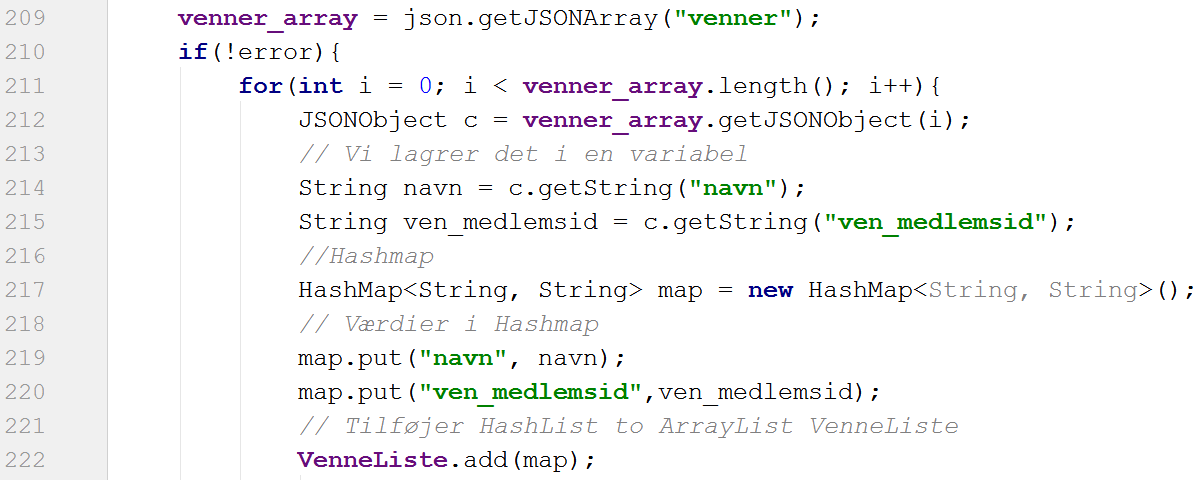
\includegraphics[width=1\textwidth]{figures/imple/vennerKode}
\caption{Udpluk af koden for venneliste. Koden viser et udpluk af, hvordan venners navn og medlemsID gemmes i arraylisten, VenneListe.}
\label{fig:vennerKode}
\end{figure} 

Af koden i figuren er der opsat en for-loop hvori JSON objekter hentes fra alle palceringerne i venner$\_$array. Hvert af disse objekter repræsentere en af brugerens venner, hvor værdier for navn og ven$\_$medlemsid hentes for disse. 
Af for-loopen ses det, at objekterne gemmes i et nyt array af navnet VenneListe, som senere benyttes til at vise vennerne i ListView for grænsefladen. Grundet bruget af HashMap til at håndtere navn og medlemsID, har det været nødvendigt at håndtere medlemsID som en string. Dette skyldes, at ved instansiering af Hashmappet defineres indputtyperne som string, idet navnet kun kan være af typen string. 

Der er i app'en mulighed for at tilføje og fjerne brugere fra vennelisten. Muligheden for at tilføje en bruger til vennelisten er implementeret ved at benytte SQL-kommandoen, der ses af \autoref{fig:opretVenKode}.

\begin{figure} [H]
\centering
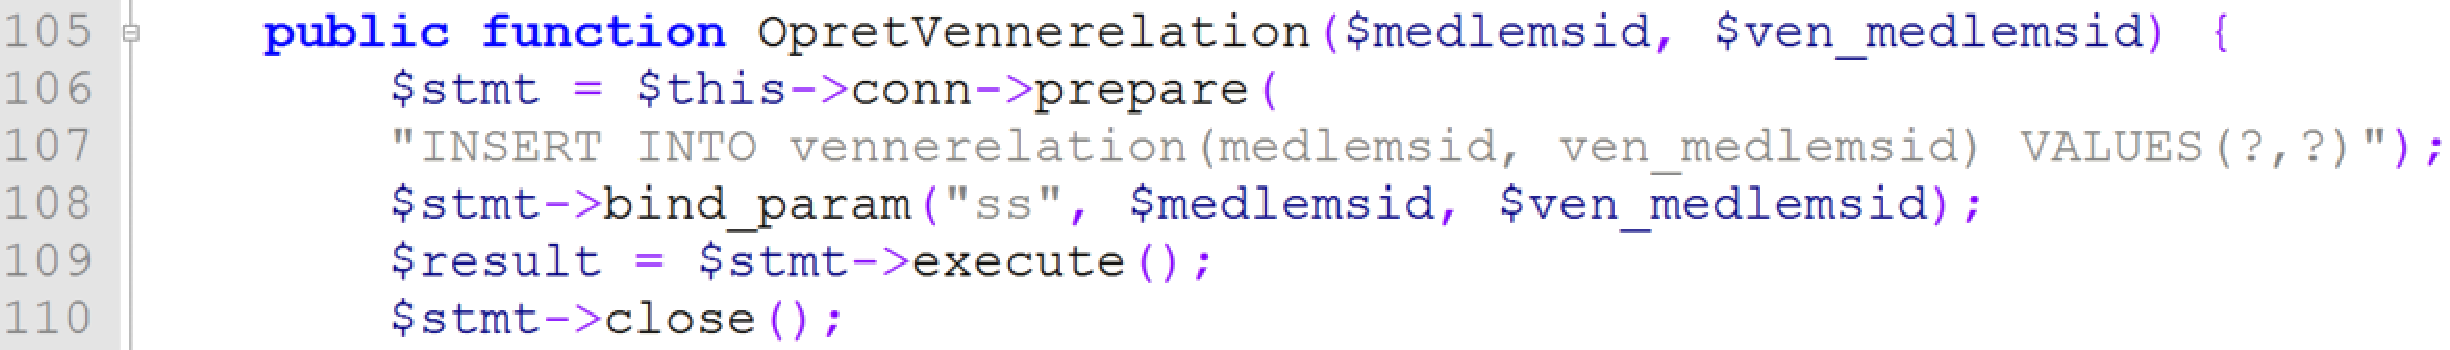
\includegraphics[width=1\textwidth]{figures/imple/opretVenKode}
\caption{SQL-kommando for tilføj bruger til venneliste.}
\label{fig:opretVenKode}
\end{figure}

I ovenstående kode ses det, at medlemsid og ven$\_$medlemsid indsættes i tabellen Vennerelation, hvorved der dannes en vennerelation. Fjernes en bruger fra vennelisten, anvendes SQL-kommandoen, der fremgår af \autoref{fig:fjernVenKode}. Dertil er forskellen fra at oprette en vennerelation, at SQL-kommandoen anvender delete, og dermed fjerner vennerelationen fra tabellen i databasen. Hertil fjernes relationen kun der, hvor både medlemsID for bruger og ven indgår. 

\begin{figure} [H]
\centering
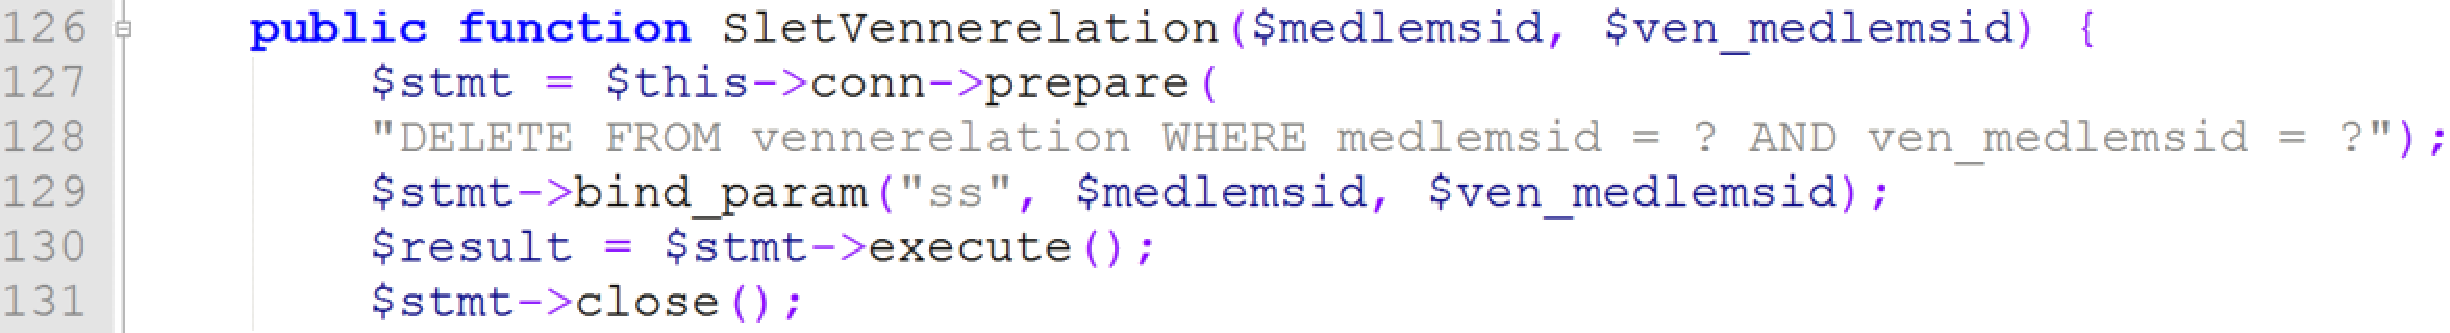
\includegraphics[width=1\textwidth]{figures/imple/fjernVenKode}
\caption{SQL-kommando for fjern bruger til venneliste.}
\label{fig:fjernVenKode}
\end{figure}

